\section*{Úvod a~cíle}
\addcontentsline{toc}{section}{\protect\numberline{}Úvod a~cíle}
Mým vybraným tématem pro seminární práci z~předmětu 3PE112 -- Podniková ekonomika pro informatiky a~statistiky je zakladatelský rozpočet pro zamýšlený podnik. Při jedné návštěvě v~mé rodině zazněl originální nápad o~založení firmy, která bude provozovat rozvoz vietnamských jídel, jelikož v~rodině máme prokazatelně šikovné kuchaře. Dalším důvodem bylo, že v~současné době, kdy se stává vietnamská kuchyně velmi oblíbenou stále více a~více lidí v~České republice, bylo by fajn využít této příležitosti k~novému podnikání. Cílem této práce je sestavit podnikový finanční rozpočet, ze kterého lze poznat, jestli je pro případ založení podniku reálné a~smysluplné provozovat zmíněnou službu.





\section{Podnikatelský záměr}
Budeme tedy provozovat cateringovou službu, která bude mít název \uv{Papajas Delivery}. Hlavní činnosti služby jsou vaření a~rozvoz čerstvých exotických obědů po hl. m. Praze. Chceme nabízet rozvoz obědů pracovníkům, kteří nemají čas chodit ven na oběd v~poledne. Budeme se specializovat především v~kvalitní výrobě a~rovněž rychlém a~spolehlivém dodání cenově dostupných výrobků, které přispívají ke zdravé výživě a~jsou základem pro zdravou stravu, dostatek energie pro práci stále většího počtu zájemců v~Praze.

\subsection{Zaměření}
Služba bude z~důvodu nedostatku pracovních sil zpočátku zaměřena pouze na velká kancelářská střediska, jako jsou Skanska, Chodov Office Park, Kavčí hory, Gemini atp. Většina velkých kancelářských center se nachází v~Praze 4, proto si zvolíme kancelář a~místo vaření na okraji jižně od Prahy, konkrétně v~Jesenicích, odkud je velmi dobrá doprava k~vybraným destinacím, jelikož budeme rozvážet vlastním nakoupeným automobilem. 

Pro začínající podnik je důležité optimalizovat náklady\index{náklad} a~tím minimalizovat případnou ztrátu. Nájem provozního prostoru na okraji Prahy je proto dobrým tahem a~taky protože bude potřeba vestavět novou kuchyň.

\subsection{Provoz}
Procházíme informační dobou. Víme, že originální nápad a~technologie jsou nezbytným základem úspěchu, proto budeme využívat výhody internetu. Objednávky se budou při\-jímat prostřednictvím webové aplikace, která bude rovněž poskytovat důležité informace pro náš podnik. Objednávky přes telefon jsou též možné. Zdrojem příjmů tedy budou objednávky obědů, jejichž ceny budou zahrnovat i~dopravné.

Budeme potřebovat minimálně tři pracovníky. Jednoho kuchaře, jednoho pomocníka a~jednoho až dva řidiče na rozvoz. V~prvním roce po zahájení budeme předpokládat tři zaměstnance s~tím, že denně budeme očekávat množství objednávek v~rozmezí 50 až 100 obědů. Ceny obědů budou stanoveny v~další kapitole.





\section{Počátek} \label{sec_pocatek}
Před zahájením si budeme muset zajistit prostor a~kuchyňská vybavení pro vaření. Cena pronájmu prostoru o~celkové velikosti 80~m$^2$ by činila 14~000~Kč/měsíc. Prostor bude dostatečně velká pro kuchyň i~menší kancelář. Kancelář bude sloužit ke sledování objednávek a~vytištění informací pro pracovníky. Předpokládaná cena za využití plynu, elektřiny a~vody je díky nenáročnosti provozu přijatelná, a~to 8~000~Kč/měsíc. Cena za ostatní služby a~náležitosti (odpad, zabezpečení, účetnictví, \ldots) by činila 3~000~Kč/měsíc.

\subsection{Náklady\index{náklad}}
Náš prostor bude pochopitelně potřebovat úpravu (odvzdušení, přívod plynu, vody) a~ná\-sledně naplnit nábytkem a~kuchyňskými spotřebiči. Do kanceláře potřebujeme internet, počítač a~tiskárnu. Dále je potřeba pro rozvoz pořídit dodávkové auto. Tabulka \ref{pocatecni_naklady} popisuje seznam předpokládaných potřebných investic do naší kuchyně a~rozvozu (v Kč).

\begin{table}[htbp]
\begin{center}
\begin{tabular}{ l r }

\textbf{Položka}&\textbf{Pořizovací cena celkem} \\ \hline 
Rekonstrukce & 200 000 \\ 
Dřevěný nábytek & 35 000 \\ 
Regály & 10 000 \\ 
Elektrické spotřebiče & 50 000 \\ 
5 $\times$ plynové vařiče & 25 000 \\ 
Nádobí, nože a~pomůcky & 10 000 \\ 
Hygienické vybavení & 5 000 \\ 
Balící souprava & 10 000 \\ 
Další pomůcky & 5 000 \\ 
Počítač, tiskárna & 25 000 \\ 
Webová aplikace na míru & 60 000 \\ 
Dodávkové auto & 300 000 \\ 
Počáteční zásoba, suroviny & 50 000 \\ \hline 
\textbf{Celkem} & \textbf{785 000} \\

\end{tabular}
\caption{Počáteční náklady\index{náklad}}
\label{pocatecni_naklady}
\end{center}
\end{table}

\subsection{Pracovní doba a~platy zaměstnancům}
Budeme se zaměřovat pouze na dodání obědů. Objednávky musí být zadány alespoň do 17h den předem. To znamená, že vařit se bude pouze ráno a~rozvážet se bude v~poledne. Odpoledne se bude uklízet a~připravovat na další den. Jelikož se o~víkendu většinou nepracuje, objednávky se budou přijímat pouze na pondělí až pátek. Pracovní doba tedy bude cca od 7h do 15h, tedy 8 hodin denně, 5 dní v~týdnu. Nebudeme uvažovat svátky.

Kuchař bude mít vzhledem k~jeho zkušenostem nejvyšší plat 30~000~Kč/měsíc, pomocník 15~000~Kč/měsíc a~řidič 15~000~Kč/měsíc. Mzdy\index{mzda} budou takto stanoveny, neboť budou všichni zaměstnanci se navzájem pomáhat. Řidič nebude pouze rozvážet, ale také se bude podílet na přípravu jídel (např. balení).





\section{Zahájení činnosti}
Náklady\index{náklad}, které budou jednorázově vynaloženy před zahájením, vyplývá z~tabulky v~kapitole \ref{sec_pocatek}, celkem tedy 785~000~Kč. Dále musíme počítat i~s~měsíčními náklady\index{náklad}, tj. provozní a~mzdové náklady\index{náklad}.


\begin{table}[htbp]
\begin{center}
\begin{tabular}{ l r l }

\textbf{Měsíční náklady\index{náklad}} & \textbf{Celkem} & \textbf{Detail} \\ \hline 
Nájemné & 14 000 & \\ 
Energie (plyn, elektřina, voda) & 8 000 & $5000 + 2200 + 800$ \\ 
Služby & 3 000 & odvoz odpadu, alarm, kamery, účetnictví\\ 
Doména a~hosting + internet & 900 & $1200 \div 12 + 300 + 500$ \\ 
Mobilní tarif k internetu & 300 & \\ 
Pohonná hmota & 4 290 & $26 \times 5 \times 33$ \\ 
Suroviny & 52 000 & $26 \times 2 000$ \\ 
Materiály & 5 200 & $26 \times 200$ \\ 
Mzdy\index{mzda} & 60 000 & $30000 + 15000 + 15000$ \\ 
Zdravotní a~sociální pojištění & 21 000 & $0,35 \times 60 000$ \\ 
Pojištění rizik a~majetku & 1 000 & $12 000 \div 12$\\ \hline 
\textbf{Celkem měsíčně} & \textbf{169 690} & \\ 
\textbf{Celkem ročně} & \textbf{2 036 280} & \\

\end{tabular}
\caption{Průběžné náklady\index{náklad}}
\label{prubezne_naklady}
\end{center}
\end{table}

\subsection{Počáteční rozvaha\index{rozvaha}}
Jsme schopni do podniku vložit 1~200~000~Kč vlastního kapitálu. Zbytek financí, na který je třeba pořídit bankovní úvěr\index{úvěr}, můžeme dopočítat z~rozvahy. Peníze na bankovním účtu slouží k~vyplacení mezd\index{mzda}, úhradě pojištění, faktur za energie a~služby, zboží, úvěrových splátek, rekonstrukce. Tento účet bude také sloužit pro příjem bezhotovostních platbeb.

\begin{table}[htbp]
\begin{center}
\begin{tabular}{ l r l r }

\multicolumn{2}{ c }{\textbf{Aktiva}\index{aktiva}} & \multicolumn{2}{ c }{\textbf{Pasiva}\index{pasiva}} \\ \hline
\textbf{Dlouhodobý hmotný majetek} & & \textbf{Vlastní kapitál} & \\
\hspace{0.5cm} Dodávkové auto & 300 000 & \hspace{0.5cm} Vklad společníků & 1 200 000 \\
\hspace{0.5cm} Kuchyňská vybavení & 675 000 & & \\

\textbf{Dlouhodobý nehmotný majetek} & & \textbf{Cizí kapitál} & \\
\hspace{0.5cm} Webová aplikace & 60 000 & \hspace{0.5cm} Bankovní úvěr\index{úvěr} & 700 000 \\

\textbf{Oběžná aktiva} & & & \\
\hspace{0.5cm} Zásoba & 110 000 & & \\
\hspace{0.5cm} Hotovost & 155 000 & & \\
\hspace{0.5cm} Bankovní účet & 600 000 & & \\ \hline
\textbf{Celkem aktiv} & \textbf{1 900 000} & \textbf{Celkem pasiv} & \textbf{1 900 000} \\

\end{tabular}
\caption{Počáteční rozvaha\index{rozvaha}}
\label{pocatecni_rozvaha}
\end{center}
\end{table}

\subsection{Bankovní úvěr\index{úvěr}}
Z~rozvahy\index{rozvaha} je patrné, že budeme muset najít půjčku za 700~000~Kč. Šlo by o~relativně malý úvěr\index{úvěr}, který bychom mohli rychle zajistit v~kterékoli bance. Jelikož máme dobrou zkušenost s~Českou spořitelnou~a.~s., budeme u~nich hledat. V~současné době ČSAS nabízí výhodné rychlé půjčky. Podle kalkulačky na stránkách České spořitelny by se úroková sazba za půjčku 700~000~Kč na dobu 5 let mohla činit 5,8~\% a~měsíční splátka by byla konstantních 13~881~Kč. Roční vývoj splácení (umořovací\index{umořovací schéma} schéma \cite{kubicek}), ze kterého jsou patrné roční úrokové náklady\index{náklad}, bude vypadat následovně:

\begin{table}[htbp]
\begin{center}
\begin{tabular}{ l r r r r r r }

\textbf{Rok} & \textbf{0.} & \textbf{1.} & \textbf{2.} & \textbf{3.} & \textbf{4.} & \textbf{5.} \\ \hline
Úrok & 0 & 40 600 & 32 480 & 24 360 & 16 240 & 8 120 \\
Úmor & 0 & 140 000 & 140 000 & 140 000 & 140 000 & 140 000 \\
Splátka & 0 & 180 600 & 172 480 & 164 360 & 156 240 & 148 120 \\ \hline
\textbf{Zůstatek} & \textbf{700 000} & \textbf{560 000} & \textbf{420 000} & \textbf{280 000} & \textbf{140 000} & \textbf{0} \\

\end{tabular}
\caption{Umořovací schéma\index{umořovací schéma}}
\label{umorovaci_schema}
\end{center}
\end{table}

%V prvním roce tedy bude činit splátka 180~600~Kč. Ta se bude skládat ze 40~600~Kč úroku a~140~000 Kč úmoru.

\newpage



\section{Vývoj podnikání}
Jediným zdrojem příjmů jsou objednávky obědů. Naše služba bude nabízet na webových stránkách pestré menu. Nyní již máme vymyšlených přes 20 jídel. Ceny se budou pohybovat v~rozmezí 60 až 110~Kč včetně dopravné. Drtivou většinu pokrmů budou tvořit 110~Kč položky, tj. hlavní jídla (rýže, pho, nudle). Ukázkové menu:

\begin{table}[htbp]
\begin{center}
\begin{tabular}{ l r | l r }

\textbf{Jídlo} & \textbf{Cena} & \textbf{Jídlo} & \textbf{Cena} \\ \hline
Jarní závitky & 60 Kč & Pho ga & 110 Kč \\ 
Letní závitky & 65 Kč & Nudle s~krevetami & 110 Kč \\ 
Hovězí na ananasu & 110 Kč & Kuřecí kari & 110 Kč \\ 
Kuřecí s~kešu & 110 Kč & Bun nem & 110 Kč \\ 
Pho bo & 110 Kč & Restovaná rýže s~kuřecím & 110 Kč \\ 
Kuřecí s~citronovou trávou & 110 Kč & Tofu v~rajčatové omáčce & 110 Kč \\ 
Krevetový salát s~nudlemi & 110 Kč & Hovězí s~fazolovými lusky & 110 Kč \\ 

\end{tabular}
\caption{Jídelní menu}
\label{jidelni_menu}
\end{center}
\end{table}

\subsection{Tržby}
Přestože je náš podnikatelský záměr originální, situace trhu je bohužel pro nás zatím nepříznivá, protože vaříme asijské obědy v~evropské zemi. Znamená to, že i~když se budeme snažit vynikat kvalitou provedení a~ručit zdravou výživu, naše produkty nemusejí být vítány českou komunitou, protože popularita exotických pokrmů v~současné době není příliš velká, aneb jen začíná stoupat. Z~tohoto důvodu budeme v~prvním roce provozu předpokládat pomalou růst ve výnosu\index{výnos}. V~letních měsících mohou tržby výrazně klesat kvůli hromadným dovoleným. Přibližný vývoj tržeb v~prvních měsících fungování bude naznačen na následujícím grafu.

\begin{figure}[htbp]
\pgfplotsset{ignore zero/.style={%
  #1ticklabel={\ifdim\tick pt=0pt \else\pgfmathprintnumber{\tick}\fi}
}}
\pgfplotsset{width=14.8cm,height=6cm}
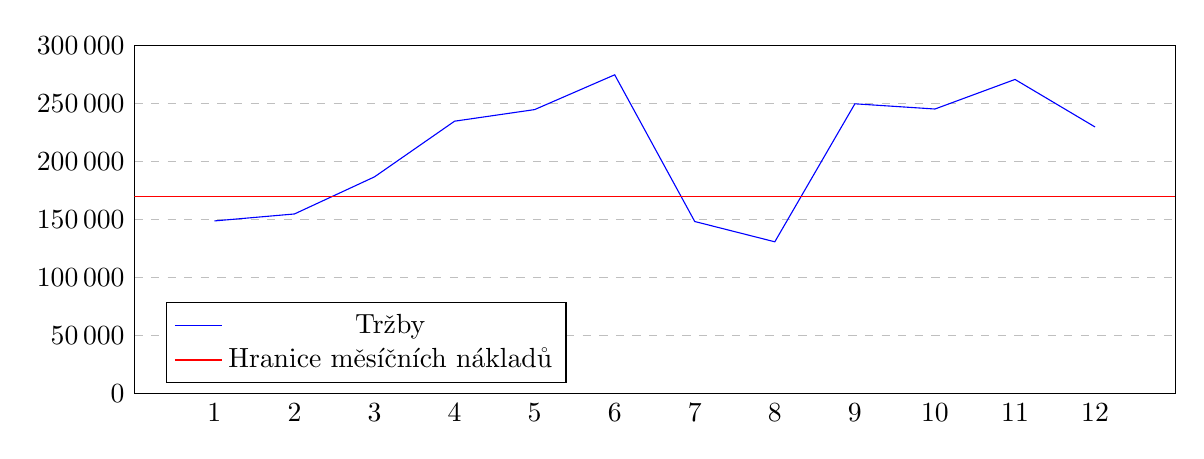
\begin{tikzpicture}%[trim axis left]
\begin{axis}[
    title={},
    xlabel={},
    ylabel={},
    xmin=0, xmax=13,
    ymin=0, ymax=300000,
    xtick={0, 1, 2, 3, 4, 5, 6, 7, 8, 9, 10, 11, 12},
    scaled y ticks = false,
    y tick label style={
        /pgf/number format/fixed,
        /pgf/number format/1000 sep=\thinspace},
    ytick={0, 50000, 100000, 150000, 200000, 250000, 300000},
    legend pos=south west,
    ymajorgrids=true,
    grid style=dashed,
    ignore zero=x,
    ytick style={draw=none},
    xtick style={draw=none},
    %nodes near coords,
    %every node near coord/.append style={rotate=90, anchor=west}
]
 
\addplot[
    color=blue,
    mark=circle,
    ]
    coordinates {
    %(0,0)
    (1,149000)
    (2,155000)
    (3,187000)    
    (4,235000)
    (5,245000)
    (6,275000)
    (7,148500)
    (8,131000)
    (9,250000)
    (10,245500)
    (11,271000)
    (12,230000)
    };
    \addlegendentry{Tržby}
    
\addplot[color=red]
    coordinates {
    (0,169690)(13,169690)
    };
    \addlegendentry{Hranice měsíčních nákladů\index{náklad}}
 
\end{axis}
\end{tikzpicture}
\caption{Předpokládaný vývoj tržeb}
\label{vyvoj_trzeb}
\end{figure}

Výše tržeb vycházejí z~počtu objednávek. Budeme uvažovat pouze 110~Kč objednávky. Denně by se dalo očekávat celkem 50 až 100 objednávek, měsíčně tedy cca přes 1300 obědů a~průměrná denní tržba by byla přes 8~000~Kč. Záleží také ale na tom, v~jakém měsíci budeme začínat. Na obrázku \ref{vyvoj_trzeb} je znázorněn případ zahájení činnosti v~lednu. Bude chvíli trvat, než se dostaneme do fáze stability. V~prvních měsících bude pro nás ztráta bohužel nevyhnutelná. Jedná se o~tzv. hladovou trasu\index{hladová trasa} fáze růstu podniku, kdy jsou výdaje výrazně větší než příjmy.

\subsection{Daňové odpisy\index{odpis}}
Odepisovat budeme všechen dlouhodobý majetek, jelikož vše bylo pořízeno nově. Skládá se z~odpisů dodávkového automobilu a~vybavení v~pronajatém prostoru a~také webové aplikace jako nehmotný dlouhodobý majetek. Nábytek, nádobí a~pomůcky činí 60~000~Kč, stroje 85~000~Kč, software 60~000~Kč. Odpisová sazba vychází z~následující tabulky:

\begin{table}[htbp]
\begin{center}
\begin{tabular}{ r l r r }
\textbf{Skupina} & \textbf{Doba} & \textbf{V 1. roce} & \textbf{V dalších letech} \\ \hline
1                & 3 roky        & 20 \%              & 40 \%                     \\ 
2                & 5 let         & 11 \%              & 22,25 \%                  \\
3                & 10 let        & 5,5 \%             & 10,5 \%                    
\end{tabular}
\caption{Odpisové sazby \cite{andrejs}}
\label{odpisove_sazby}
\end{center}
\end{table}

Pro dlouhodobý nehmotný majetek, tedy náš objednávkový systém, kterou bychom koupili za 60~000~Kč, bude platit rovnoměrný 3letý odpis\index{odpis}, jelikož 60~000~Kč je dolní hranice vstupní ceny nehmotného majetku. Ročně tedy činí odpis\index{odpis} softwaru $60~000 \div 3 = 20~000~\text{Kč}$. Nebudeme počítat s~žádným technickým zhodnocením\index{zhodnocení} jako je upgrade apod. V~prvním roce budeme aplikovat rovnoměrné odpisy\index{odpis} následovně:

\begin{table}[htbp]
\begin{center}
\begin{tabular}{lrlrrr}
\textbf{Majetek} & \textbf{Skupina}     & \textbf{Doba} & \textbf{Vstupní cena} & \textbf{1. koeficient}               & \textbf{1. odpis\index{odpis}} \\ \hline
Dodávkové auto   & 2                    & 5 let         & 300 000               & 11                                   & 33 000            \\
Nábytek a~stroje & 2                    & 5 let         & 145 000               & 11                                   & 15 950            \\
Webová aplikace  & -                    & 3 roky        & 60 000                & -                                    & 20 000            \\ \hline
                 & \multicolumn{1}{l}{} &               & \multicolumn{2}{r}{Celkem odpis\index{odpis} za 1. rok} & \textbf{68 950}           
\end{tabular}
\caption{Daňové odpisy\index{odpis}}
\label{danove_odpisy}
\end{center}
\end{table}




\section{Výsledky}

Po prvním roce se očekává účetní výsledek, který má vypovídat o~tom, zda se bude jednat o~zisk či ztrátu. Budeme optimističtí.

\subsection{Výsledovka ke konci prvního roku po zahájení}
Sazba daně z~příjmů fyzických osob v~České republice činí 15~\%. Daň musíme pak na konci ještě odečíst z~výsledku hospodaření, abychom měli čistý zisk (EAT\index{EAT}).

\begin{table}[htbp]
\begin{center}
\begin{tabular}{lllr}
%\multicolumn{4}{c}{\textbf{Výsledovka ke konci prvního roku provozu}}                                        \\
\multicolumn{2}{c}{\textbf{Výnosy}\index{výnos}}                    & \multicolumn{2}{c}{\textbf{Náklady\index{náklad}}}                \\ \hline
Tržby z~prodeje        & \multicolumn{1}{r}{2 522 000} & Rekonstrukce                   & 200 000            \\
                       & \multicolumn{1}{r}{}          & Nájem                          & 60 000             \\
                       &                               & Energie                        & 96 000             \\
                       &                               & Služby                         & 36 000             \\
                       &                               & Doména, hosting, internet      & 10 800             \\
                       &                               & Mobilní tarif                  & 3 600              \\
                       &                               & Pohonná hmora                  & 51 480             \\
                       &                               & Suroviny                       & 624 000            \\
                       &                               & Materiály                      & 62 400             \\
                       &                               & Mzdy\index{mzda}                           & 720 000            \\
                       &                               & Zdravotní a~sociální pojištění & 252 000            \\
                       &                               & Pojištění rizik a~majetku      & 12 000             \\
                       &                               & Úrokové náklady\index{náklad}                & 40 600             \\
                       &                               & Odpisy\index{odpis}                         & 68 950             \\ \hline
\textbf{Celkem výnosy}\index{výnos} & \textbf{2 522 000}            & \textbf{Celkem náklady\index{náklad}}        & \textbf{2 345 830} \\
\textbf{Ztráta}        & \textbf{0}                    & \textbf{Zisk před zdaněním}    & \textbf{176 170}   \\
                       &                               & \textbf{Daň z~příjmu 15 \%}    & \textbf{26 426}    \\
                       &                               & \textbf{Zisk po zdanění}       & \textbf{149 744}  
\end{tabular}
\caption{Výsledovka ke konci prvního roku}
\label{vysledovka}
\end{center}
\end{table}

\newpage

\subsection{Rozvaha\index{rozvaha} ke konci prvního roku po zahájení}
Nájemné se bude platit na fakturu a~vždy do 15.~dne následujícího měsíce bezhotovostním převodem. To samé bude platit u~faktur za energie, služby, doména, hosting, internet, mobilní tarif a~pojištění rizik. Mzdy\index{mzda} budou vypláceny též měsíc zpětně, a~to bezhotovostně na účty zaměstnanců, současně se bude platit i~zdravotní a~sociální pojištění k~danému měsíci. Zásobu a~materiál budeme mít zajištěné každý měsíc od dodavatele asijských potravin a~gastronomicky specializovaného dodavatele a~to vše na fakturu se splatností 14~dnů. 

Hotovost slouží mimo jiné hlavně k~menších nákupů zelenin, syrového masa a~přísad ve velkoobchodech. V~průběhu roku by se určitě muselo dojít k~vkládání hotovosti z~tržeb na bankovní účet, ze kterého budou odcházet průběžné výdaje. Pasivum dodavatelé zahrnuje veškeré nezaplacené faktury za služby či zboží včetně nájemné, tj. závazky k~dodavatelům.

\begin{table}[htbp]
\begin{center}
\begin{tabular}{ l r l r }

\multicolumn{2}{ c }{\textbf{Aktiva}\index{aktiva}} & \multicolumn{2}{ c }{\textbf{Pasiva}\index{aktiva}} \\ \hline
\textbf{Dlouhodobý hmotný majetek} & & \textbf{Vlastní kapitál} & \\
\hspace{0.5cm} Dodávkové auto & 300 000 & \hspace{0.5cm} Vklad společníků & 1 200 000 \\
\hspace{0.5cm} Kuchyňská vybavení & 675 000 & \hspace{0.5cm} VHBO po zdanění & 149 744 \\
\hspace{0.5cm} -oprávky & $-48~950$ & & \\
\\
\textbf{Dlouhodobý nehmotný majetek} & & \textbf{Cizí kapitál} & \\
\hspace{0.5cm} Webová aplikace & 60 000 & \hspace{0.5cm} Bankovní úvěr\index{úvěr} & 560 000 \\
\hspace{0.5cm} -oprávky & $-20~000$ & \hspace{0.5cm} Daňový dluh & 26 426 \\
& & \hspace{0.5cm} Dluhy SP a~ZP & 21 000 \\

\textbf{Oběžná aktiva} & & \hspace{0.5cm} Zaměstnanci & 60 000 \\
\hspace{0.5cm} Zásoba & 110 000 & \hspace{0.5cm} Dodavatelé & 84 400 \\
\hspace{0.5cm} Hotovost & 100 000 & & \\
\hspace{0.5cm} Bankovní účet & 925 520 & & \\ \hline
\textbf{Celkem aktiv} & \textbf{2 101 570} & \textbf{Celkem pasiv} & \textbf{2 101 570} \\

\end{tabular}
\caption{Rozvaha\index{rozvaha} po prvním roce}
\label{rozvaha_po_prvnim_roce}
\end{center}
\end{table}

\newpage

\subsection{Cashflow\index{cashflow} v~prvním roce po zahájení}
Přímou i~nepřímou metodou \cite{synek_kislingerova}:

\begin{table}[htbp]
\begin{center}
\begin{tabular}{lrllr}
\multicolumn{3}{c}{\textbf{Přímá metoda}}                               & \multicolumn{1}{c}{\textbf{Nepřímá metoda}} &                          \\ \hline
\textbf{Počáteční stav}                    & 755 000            &                   & \textbf{Počáteční stav}                           & 755 000            \\
\textbf{Příjmy}                            & 2 522 000          &                   & $+\text{Čistý zisk}$                              & 149 744            \\
\textbf{Výdaje}                            & 2 251 480          &                   & $+\text{Odpisy}$                                  & 68 950             \\
\hspace{0,5cm}Rekonstrukce                 & 200 000            &                   & $-\text{Odběratelé}$                              & 0                  \\
\hspace{0,5cm}Nájem                        & 154 000            & $11 \times 14000$ & $+\text{Dodavatelé}$                              & 84 400             \\
\hspace{0,5cm}Energie                      & 88 000             & $11 \times 8000$  & $-\text{Úmor}$                                    & $-140~000$         \\
\hspace{0,5cm}Služby                       & 33 000             & $11 \times 3000$  & $+\text{Zaměstnanci}$                             & 60 000             \\
\hspace{0,5cm}Doména, hosting              & 9 900              & $11 \times 900$   & $+\text{ZP, SP}$                                  & 21 000             \\
\hspace{0,5cm}Mobilní tarif                & 3 300              & $11 \times 300$   & $+\text{Daňový dluh}$                             & 26 426             \\
\hspace{0,5cm}Pohonná hmota                & 51 480             & $12 \times 4290$  &                                                   &                    \\
\hspace{0,5cm}Suroviny                     & 572 000            & $11 \times 52000$ &                                                   &                    \\
\hspace{0,5cm}Materiály                    & 57 200             & $11 \times 5200$  &                                                   &                    \\
\hspace{0,5cm}Mzdy\index{mzda}                         & 660 000            & $11 \times 60000$ &                                                   &                    \\
\hspace{0,5cm}Zdrav. a~soc. poj.           & 231 000            & $11 \times 21000$ &                                                   &                    \\
\hspace{0,5cm}Poj. rizik a~majetku         & 11 000             & $11 \times 1000$  & \textbf{}                                         & \textbf{}          \\
\hspace{0,5cm}Splátka úvěru\index{úvěr}                & 180 600            &                   & \textbf{}                                         & \textbf{}          \\ \hline
\textbf{Cashflow\index{cashflow}}                          & \textbf{270 520}   &                   & \textbf{Cashflow\index{cashflow}}                                 & \textbf{270 520}   \\
\textbf{Konečný stav}                      & \textbf{1 025 520} &                   & \textbf{Konečný stav}                             & \textbf{1 025 520}
\end{tabular}
\caption{Cashflow\index{cashflow} po prvním roce}
\label{cashflow}
\end{center}
\end{table}


\section{Finanční páka\index{finanční páka} a~ukazatelé rentability}
EBIT\index{EBIT} by nám vyšel $149~744 + 26~426 + 40~600 = 216~770~\text{Kč}$. Nyní si spočítáme, jak přínosný by pro nás byl úvěr\index{úvěr} za 700~000~Kč od České spořitelny, viz tabulka \ref{efekt_financni_paky}.

\begin{table}[htbp]
\begin{center}
\begin{tabular}{ l | r r }
& \multicolumn{1}{|c}{\textbf{S úvěrem}\index{úvěr}} & \multicolumn{1}{l}{\textbf{Bez úvěru}\index{úvěr}} \\ \hline
\textbf{Kapitál}              & 1 900 000                             & 1 900 000                              \\
\textbf{VK}                   & 1 200 000                             & 1 900 000                              \\
\textbf{CK}                   & 700 000                               & 0                                      \\
\textbf{EBIT\index{EBIT}}                 & 216 770                               & 216 770                                \\
\textbf{Úrok}                 & 40 600                                & 0                                      \\
\textbf{EBT}                  & 176 170                               & 216 770                                \\
\textbf{EBT na VK}            & 0,146 808                              & 0,114 089                               \\
\textbf{Daň}                  & 26 426                                & 32 516                                 \\
\textbf{EAT\index{EAT}}                  & 149 774                               & 184 254                                \\
\textbf{ROE}                  & 0,124 786                              & 0,096 975                              
\end{tabular}
\caption{Efekt finanční páky \cite{mikovcova_schollerova}\index{finanční páka}}
\label{efekt_financni_paky}
\end{center}
\end{table}

Je zde patrné, že rentabilita vlastního kapitálu by byla u~varianty s~úvěrem\index{úvěr} vyšší než u~varianty bez úvěru\index{úvěr}. Finanční páka\index{finanční páka} by působila na náš podnik pozitivně, i~když ne o~moc (cca 3~\%) výhodnější.

Rentabilita vlastního kapitálu (ROE) by byla cca 12,5~\% a~rentabilita aktiv\index{ROA} by byla $ \text{ROA} = \text{zisk} \div \text{aktiva} = 149~744 \div 2~101~570 = 7,12~\%$. Hodnoty ukazatelů rentability jsou pochopitelně nízké, jelikož jsme začínající podnik a~máme za sebou jen první \uv{zdařilý} rok podnikání.





\section{Oportunitní náklady\index{oportunitní náklady}}
\textit{Last but not least}. Zajímalo by nás, co kdybychom do tohoto podnikání nešli, je podnikání pro nás výhodnější, než když bychom pracovali jinde či investovali jinak? To si také můžeme spočítat na základě tzv. \textit{oportunitních nákladech}\index{oportunitní náklady}\cite{kubicek}, pomocí kterých lze také zjistit, zda firma dosahuje ekonomický zisk\index{ekonomický zisk}.

Mezi oportunitní náklady\index{oportunitní náklady} lze zařadit mzdu\index{mzda} vlastníka, kdyby pracoval v~jiné firmě. Dále jeho finanční úsporu, kterou by byl schopen vložit do kapitálu firmy. Tu by mohl naspořit v~bance, nejlépe přes dluhopisy\index{dluhopis}. Průměrný výnos\index{výnos} z~dluhopisů\index{dluhopis} by byl cca 5~\% za rok.

\begin{itemize}
\item měsíční plat vlastníka u~jiné firmy: 25~000~Kč
\item úspora vlastníka: 1~200~000~Kč
\end{itemize}

Celkem roční oportunitní náklady\index{oportunitní náklady}: $1~200~000 \times 0,05 + 12 \times 25~000 = 360~000~\text{Kč}$. Pokud by byl vlastník přímo kuchařem, jeho roční příjem by byl $12 \times 30~000 + 149~744 = 509~744~\text{Kč}$, což je patrně vyšší plat než u~starého zaměstnání. Je třeba konečně zde Vám čtenáři prozradit, že podnikatelský záměr byl skutečně nápad mého strýce, který pracuje jako profesionální šéfkuchař v~PHO Original restauraci v~Praze.

\newpage




\fancyhf{}
\pagestyle{fancy}

\section*{Závěr}
\addcontentsline{toc}{section}{\protect\numberline{}Závěr}
\textit{Easier said than done}. K takovému optimisticky kladnému výsledku hospodaření v~prvním roce podnikání se chtěl dopracovat každý. Aby to ale vše mohlo skutečně vyjít, alespoň tedy přibližně, je potřeba do našeho podnikového plánu zapojit mnohem více věcí a~úsilí, např. marketing je klíčový pro rozjezd služby, klást si důraz na kvalitu. Ze začátku je zásadní propagovat naši službu s~maximálním úsilím. Skutečnost je, že pokud bychom získali alespoň 20~\% zájemců o~naši službu přes rozdávání letáků před kanceláří, bylo by to i~tak velké štěstí. Pomohla by mimochodem i~propagace přes internet, tj. na sociálních sítích (Facebook, Twitter) a~pomocí reklamních kampaní (Google AdWords) či doporučení přes populární gastronomické blogy.

Nesmíme zapomenout, že naše služba je poháněna hlavně za pomocí webové aplikace. Je to místo, kde se odehrávají nejdůležitější pohyby, tj. styk se zákazníky. Je proto velmi důležité se jí věnovat a~zdokonalit její funkčnost a~přívětivost. Časem by bylo dobré najmout dalšího pracovníka, který se bude starat o~CRM. V~případě úspěchu v~prvním roce by se firmě vyplatilo nechat zhotovit mobilní aplikaci pro zpevnění vztahu se zákazníky pomocí notifikací atp. Rozhodně není zbytečné naše menu do budoucna rozšířit o~nové atraktivnější pokrmy.